\section{PINN Architecture and Training Strategy}

This section presents the general architecture and training methodology used for the Physics-Informed Neural Networks (PINNs) developed in this work. The objective is to construct a neural network capable of approximating the solution of the governing physical problem while simultaneously satisfying the underlying partial differential equation (PDE).

Unlike traditional supervised learning approaches that rely exclusively on observational data, PINNs integrate physical laws directly into the optimization process through automatic differentiation and physics-based loss functions. The neural network therefore acts as a continuous function approximator constrained by both available data and fundamental physical principles.

% =========================================================
\subsection{General Neural Network Architecture}

The temperature field is approximated by a fully connected feedforward neural network,

\begin{equation}
T_{\theta}(x,t) = \mathcal{N}_{\theta}(x,t),
\end{equation}

where

\begin{itemize}
\item $\mathcal{N}_{\theta}$ denotes the neural network,
\item $\theta$ represents the set of trainable parameters, including all weights and biases,
\item $(x,t)$ are the spatial and temporal coordinates provided as inputs.
\end{itemize}

The objective of the neural network is to learn the unknown mapping between the spatial-temporal coordinates $(x,t)$ and the corresponding temperature field $T(x,t)$. The network takes the coordinates $(x,t)$ as inputs and returns the predicted temperature value $T_{\theta}(x,t)$. The NN architecture for the 1D thermal problem is composed of

\begin{itemize}
\item an input layer containing the spatial and temporal coordinates,
\item several fully connected hidden layers, each composed of multiple neurons,
\item an output layer producing the predicted temperature field.
\end{itemize}

At the most fundamental level, a neural network is composed of interconnected computational units called neurons. Each neuron receives information from the previous layer, computes a weighted sum of its inputs, adds a bias term, and applies a nonlinear activation function. Mathematically, the output of a neuron can be expressed as

\begin{equation}
a = \sigma
\left(
\sum_i w_i x_i + b
\right),
\end{equation}

where $x_i$ are the inputs, $w_i$ are the trainable weights, $b$ is a bias term, and $\sigma(\cdot)$ denotes the activation function.

The role of a neuron can be viewed as transforming information received from the previous layer into a new representation. In the first hidden layers, neurons often learn relatively simple features of the target function, while deeper layers combine these elementary features into increasingly complex representations. Through the collective action of many neurons, the network progressively constructs an approximation of the solution $T_{\theta}(x,t)$.

For the one-dimensional heat diffusion problem considered in this work, a neuron may, for example, learn to respond preferentially to a specific region of the spatial domain or to a particular stage of the temporal evolution. Some neurons may contribute to describing the temperature gradients near the boundaries, while others may capture the global decay of temperature over time. The final temperature field is obtained by combining the contributions of all neurons through the network layers. Although such interpretations can be useful for small networks, the role of individual neurons becomes increasingly difficult to identify as the network size grows, since the learned representation is distributed across many neurons.

The specialization of neurons is not prescribed explicitly. At the beginning of training, the network parameters are initialized (see section). As the optimization progresses, the weights and biases are adjusted through backpropagation in order to minimize the loss function. Neurons therefore gradually adapt to the features that are most useful for reducing the prediction error and satisfying the physical constraints. While the initial random weights influence the early stages of training and may lead to slightly different learned representations, the final organization of the neurons is primarily driven by the optimization process rather than by the initialization itself. Consequently, two networks trained from different random initializations may use different internal neuron representations while still converging toward nearly identical temperature fields.

In a fully connected architecture, every neuron of a given layer is connected to every neuron of the following layer through trainable weights. During training, these parameters are continuously adjusted through \textit{backpropagation} so that the network progressively improves its approximation of the target solution. The weights determine how strongly each input influences the response of a neuron. Large positive weights increase the importance of a particular input, whereas small or negative weights reduce its contribution. During training, the network automatically adjusts these weights to identify the combinations of spatial and temporal coordinates that best describe the temperature field. Biases play a complementary role. While the weights control the slope and orientation of the neuron response, the bias shifts this response and determines the activation threshold of the neuron. Without biases, all neuron responses would be constrained to pass through the origin, significantly limiting the family of functions that the network can represent.

As a simple illustration, consider a neuron computing

\begin{equation}
a = \sigma(wx+b).
\end{equation}

The weight $w$ controls how rapidly the neuron reacts to variations of the input $x$, whereas the bias $b$ determines the location where the neuron becomes active. Together, weights and biases provide the flexibility required to approximate complex nonlinear functions accurately.

For the one-dimensional heat diffusion problem considered here, the weights may adapt to capture spatial or temporal variations of the temperature field, while the biases allow the corresponding features to appear at different locations in space and time. Although the influence of an individual weight or bias is generally difficult to interpret, their collective adjustment enables the network to approximate the solution of the governing physical problem. 

Although the mathematical operation performed by an individual neuron is relatively simple, the behavior of a deep neural network containing hundreds or thousands of neurons is generally difficult to interpret. While some neurons may appear to specialize in particular features, there is usually no straightforward physical meaning associated with a specific neuron. Instead, the learned representation is distributed across many neurons and layers. For this reason, neural networks are often considered as \textit{black-box} models, although considerable research efforts are currently devoted to improving their interpretability.

The number of hidden layers (depth) and the number of neurons per layer (width) are important hyperparameters that can significantly influence both the approximation capability and optimization behavior of the PINN. Increasing the width generally increases the number of features that can be represented within a layer, whereas increasing the depth enables the network to construct more complex hierarchical representations of the solution. Unlike conventional neural networks, PINNs also incorporate physical constraints through the computation of PDE residuals using automatic differentiation. These residuals are included in the loss function and guide the optimization process toward solutions that satisfy the governing physical equations.

A general illustration of the PINN architecture used throughout this work is presented in Fig.~\ref{fig:pinn_architecture}.

\begin{landscape}

\begin{figure}[p]
\centering
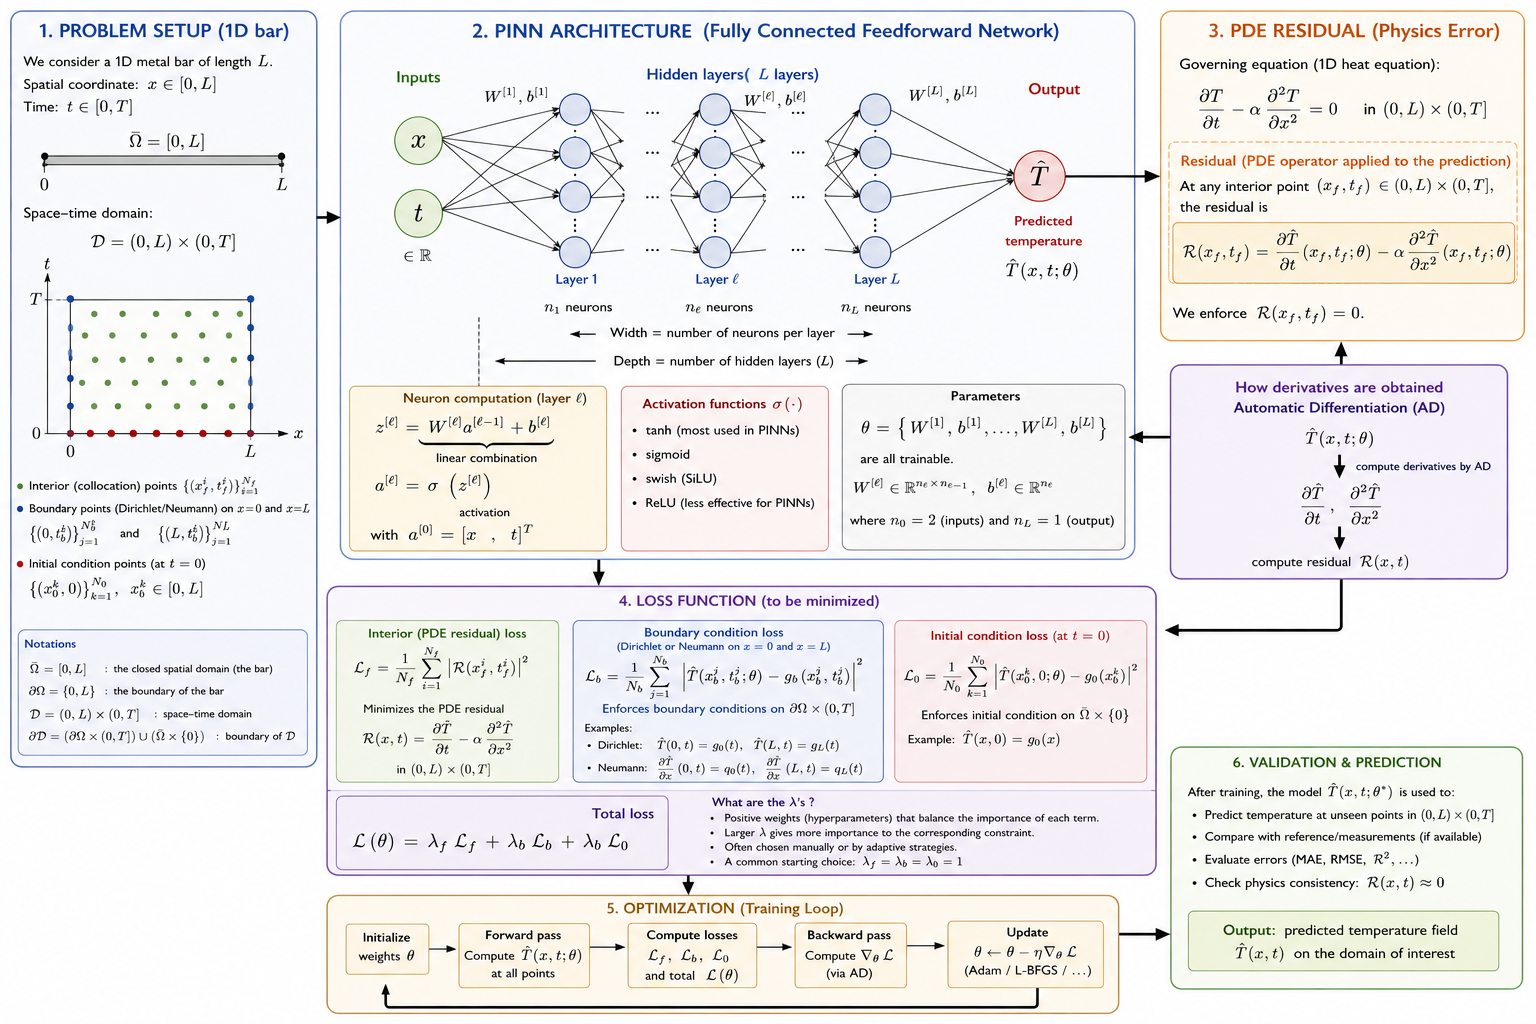
\includegraphics[
width=0.95\linewidth,
height=0.95\textheight,
keepaspectratio
]{figures/Pinn_architecture.png}
\caption{General architecture of a Physics-Informed Neural Network (PINN) applied to the one-dimensional heat equation. The network receives the spatial and temporal coordinates as inputs and predicts the temperature field. Automatic differentiation is then used to compute the PDE residual and enforce the physical constraints during training.}
\label{fig:pinn_architecture}
\end{figure}

\end{landscape}


% =========================================================
\subsection{Activation Functions}
% =========================================================

\subsection{Activation Functions and the Need for Non-Linearity}

In a neural network, each neuron first computes a weighted sum of its inputs,

\begin{equation}
z^{(\ell)} = W^{(\ell)} a^{(\ell-1)} + b^{(\ell)},
\end{equation}

where $W^{(\ell)}$ and $b^{(\ell)}$ denote the weights and biases of layer $\ell$, respectively. The result is then passed through an activation function $\sigma(\cdot)$,

\begin{equation}
a^{(\ell)} = \sigma\left(z^{(\ell)}\right).
\end{equation}

The activation function is a key component of neural networks because it introduces non-linearity into the model.

Without an activation function, every layer would simply perform a linear transformation of its inputs. Since the composition of multiple linear transformations remains linear, a deep neural network composed only of linear operations would be mathematically equivalent to a single linear layer, regardless of the number of hidden layers. In such a case, increasing the depth of the network would provide no additional learning capability.

As a simple analogy, stacking several straight rulers on top of each other still produces a straight line. To represent complex patterns, curves, and nonlinear relationships, the network must include nonlinear operations between layers.

Nonlinear activation functions allow neural networks to approximate highly complex functions and are therefore essential for solving realistic engineering and scientific problems. In fact, the Universal Approximation Theorem states that a sufficiently large neural network equipped with nonlinear activation functions can approximate a wide range of continuous functions with arbitrary accuracy.

In classical supervised machine learning, one of the most widely used activation functions is the Rectified Linear Unit (ReLU), defined as

\begin{equation}
\sigma_{\mathrm{ReLU}}(x)
=
\max(0,x)
=
\begin{cases}
0, & x < 0,\\
x, & x \ge 0.
\end{cases}
\end{equation}

The ReLU activation function is illustrated in Fig.~\ref{fig:relu}.

ReLU became popular because of its simplicity and computational efficiency. For negative inputs, the output is zero, whereas for positive inputs the function behaves linearly. This piecewise behavior helps mitigate the vanishing-gradient problem that affected earlier activation functions such as the sigmoid and hyperbolic tangent functions when training very deep networks.

Although ReLU has become the standard activation function in many machine learning applications such as image classification, natural language processing, and computer vision, it is generally not the preferred choice for Physics-Informed Neural Networks (PINNs).

The reason is that PINNs require automatic differentiation to compute first- and higher-order derivatives of the neural network output with respect to the input variables. Since the ReLU function is not differentiable at $x=0$ and has a zero second derivative almost everywhere, it often produces poor approximations of differential operators appearing in partial differential equations.

For this reason, smooth activation functions such as the hyperbolic tangent function,

\begin{equation}
\sigma(x)=\tanh(x),
\end{equation}

are commonly preferred in PINNs. Their smoothness allows accurate computation of higher-order derivatives and generally leads to better convergence when solving differential equations.

\begin{figure}[h]
    \centering
    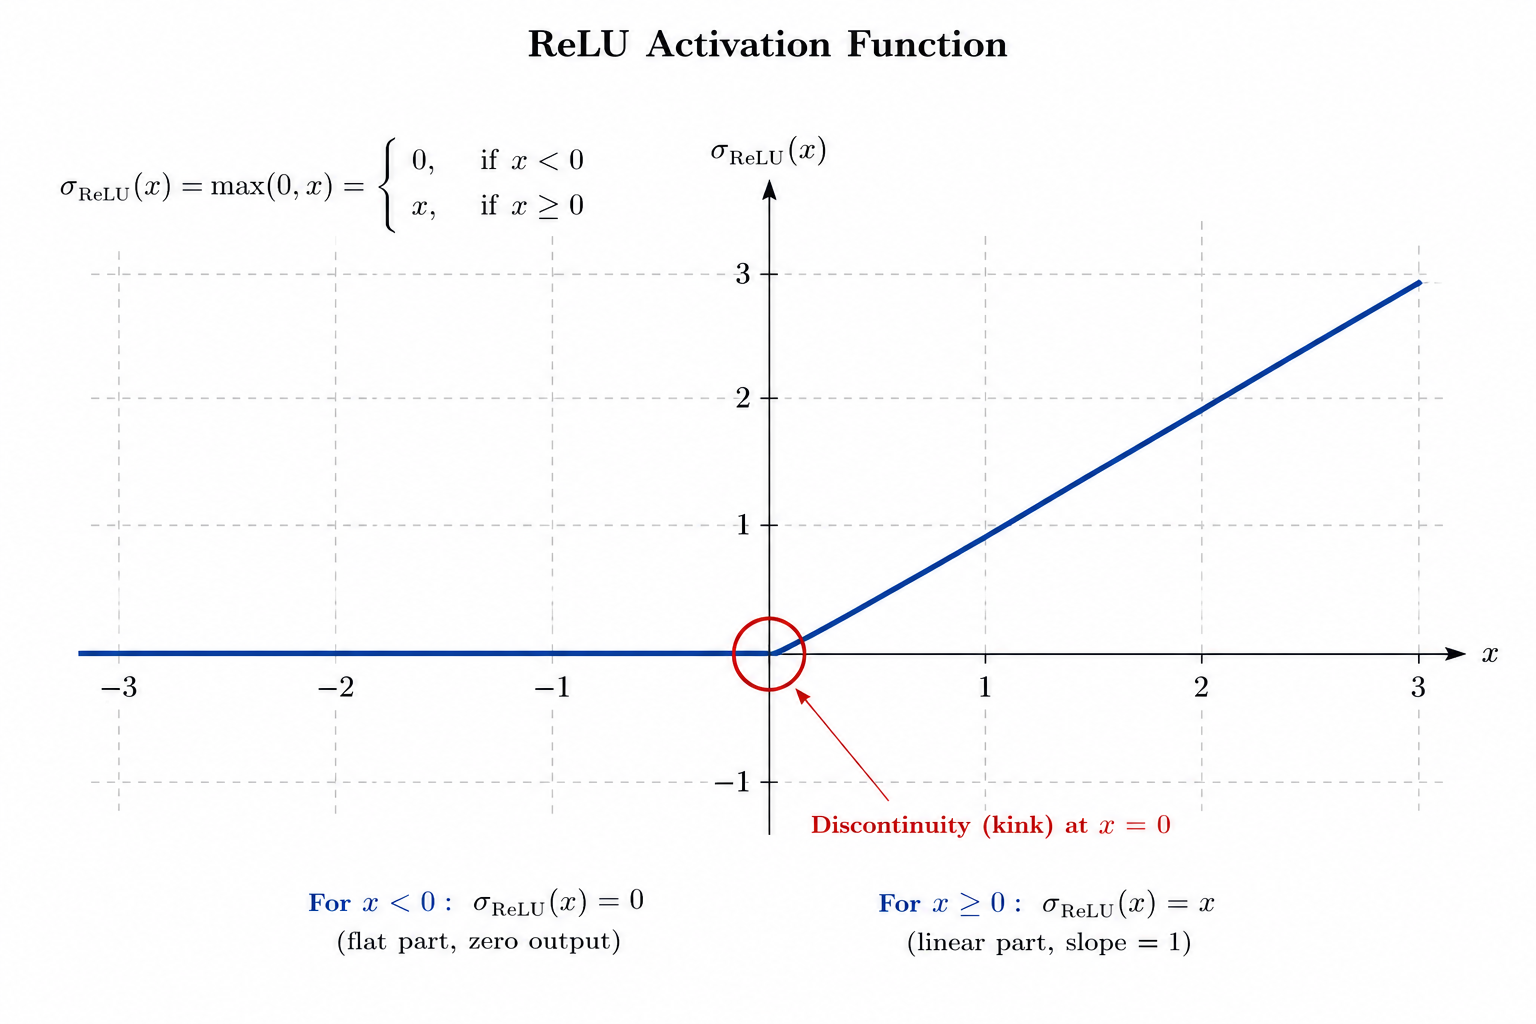
\includegraphics[width=0.75\linewidth]{figures/Relu.png}
    \caption{The Relu function}
    \label{fig:relu}
\end{figure}

In this work, the hyperbolic tangent activation function is primarily employed:

\begin{equation}
\sigma(z)=\tanh(z)
\end{equation}

The \texttt{tanh} activation is commonly used in PINN applications because:
\begin{itemize}
    \item it is smooth and infinitely differentiable,
    \item its derivatives are stable for automatic differentiation,
    \item and it generally provides better convergence properties for PDE-related problems compared to piecewise linear activations such as ReLU.
\end{itemize}

\begin{figure}[h]
    \centering
    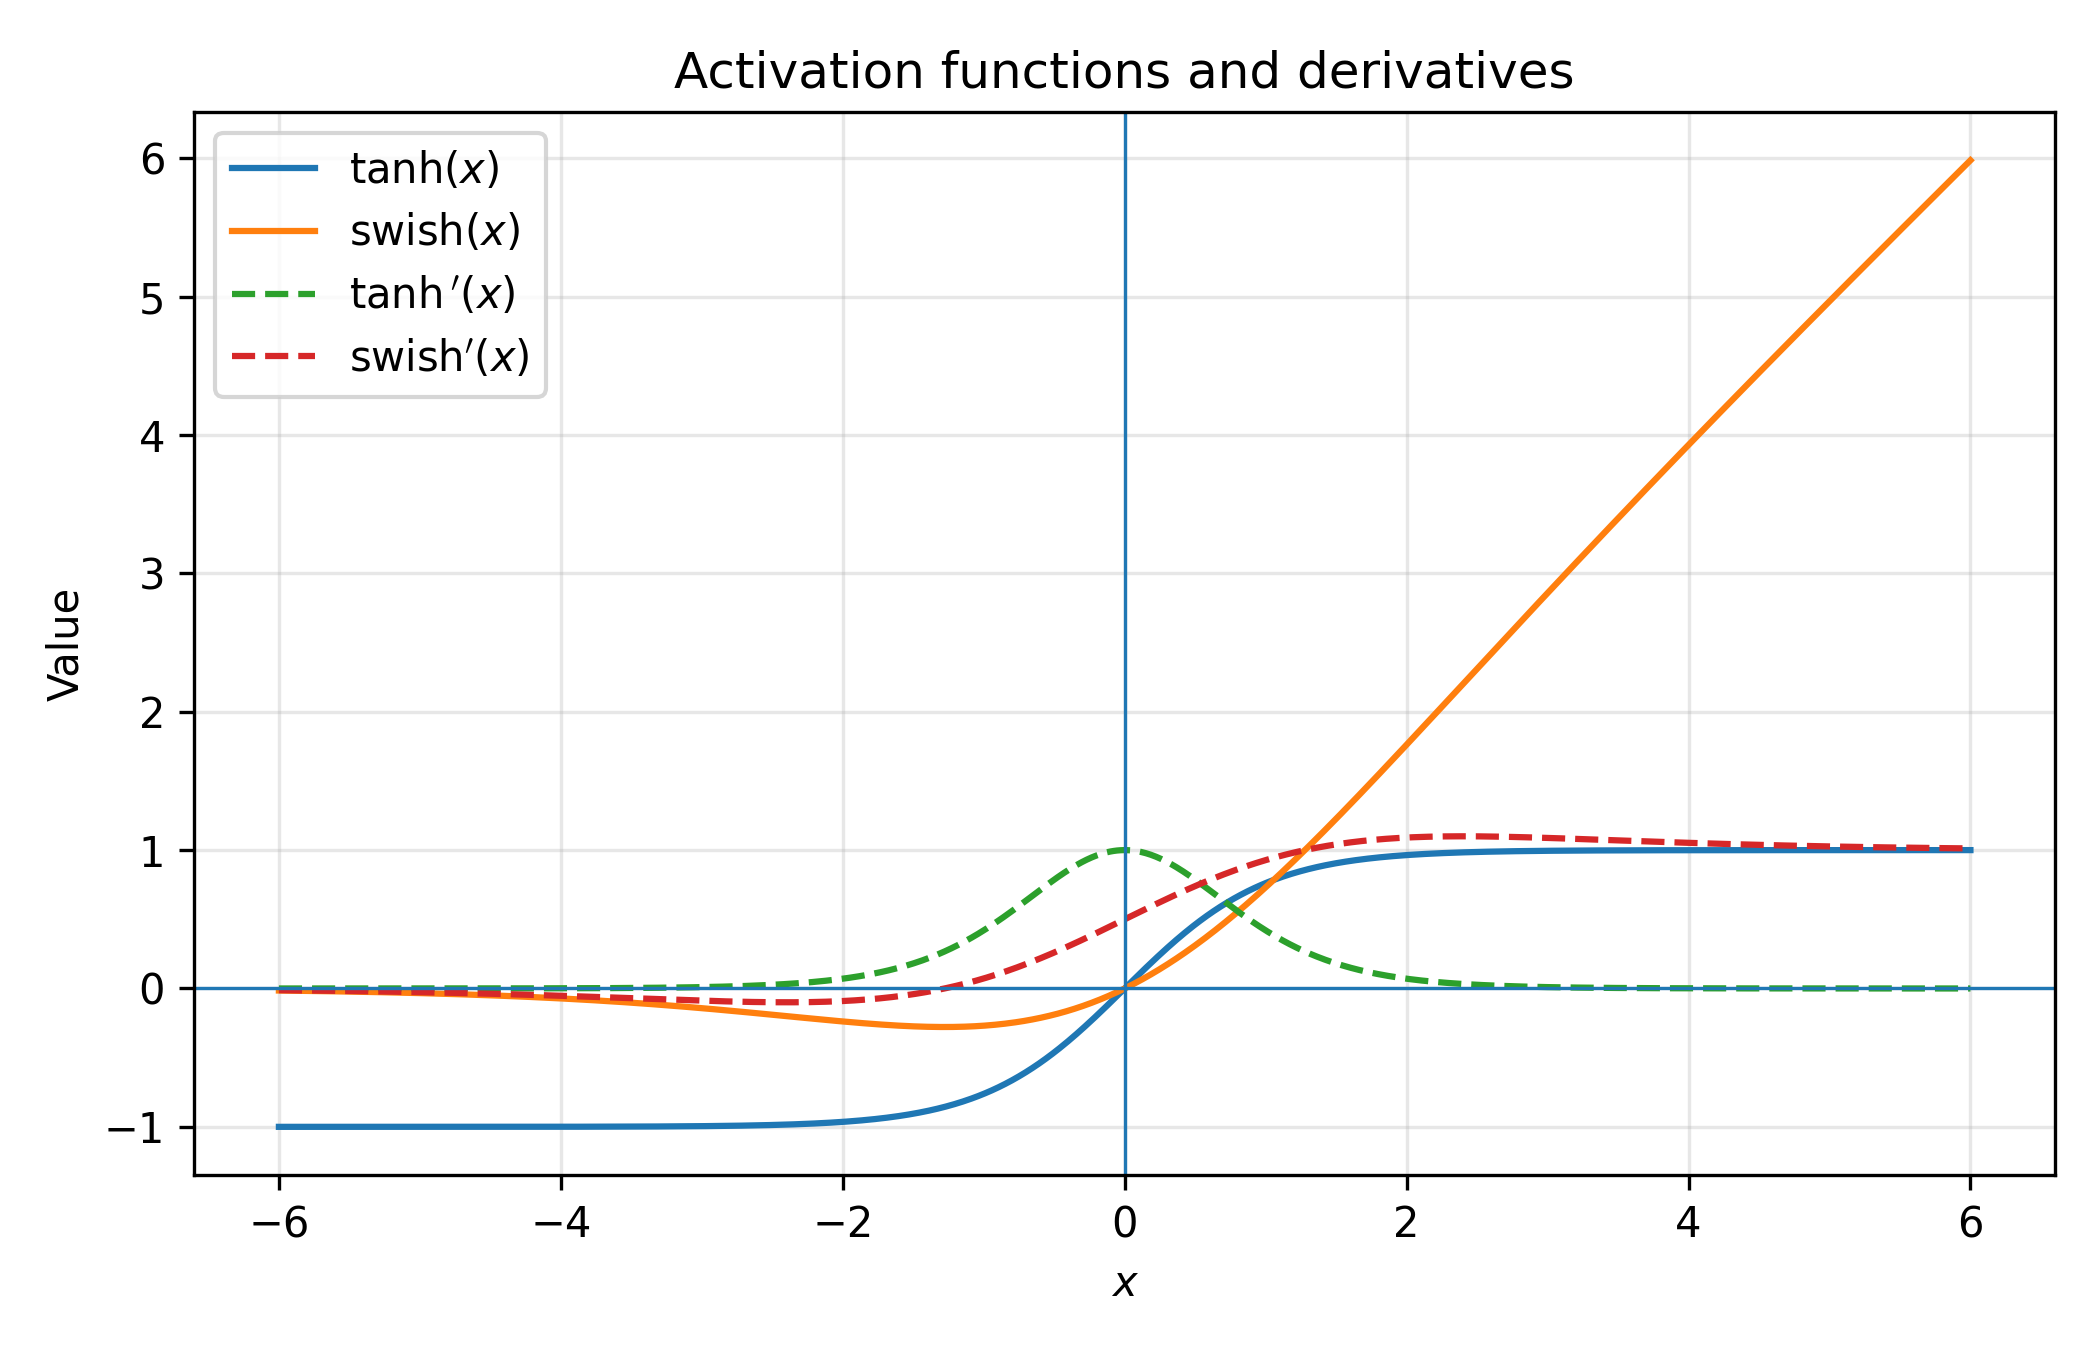
\includegraphics[width=0.75\linewidth]{figures/activation_functions_and_derivatives.png}
    \caption{Comparison of the derivatives of the \texttt{tanh} and \texttt{swish} activation functions.}
    \label{fig:activation_derivatives}
\end{figure}

A combined visualization of the activation functions and their derivatives is shown in Figure~\ref{fig:activation_combined}.

\begin{figure}
    \centering
    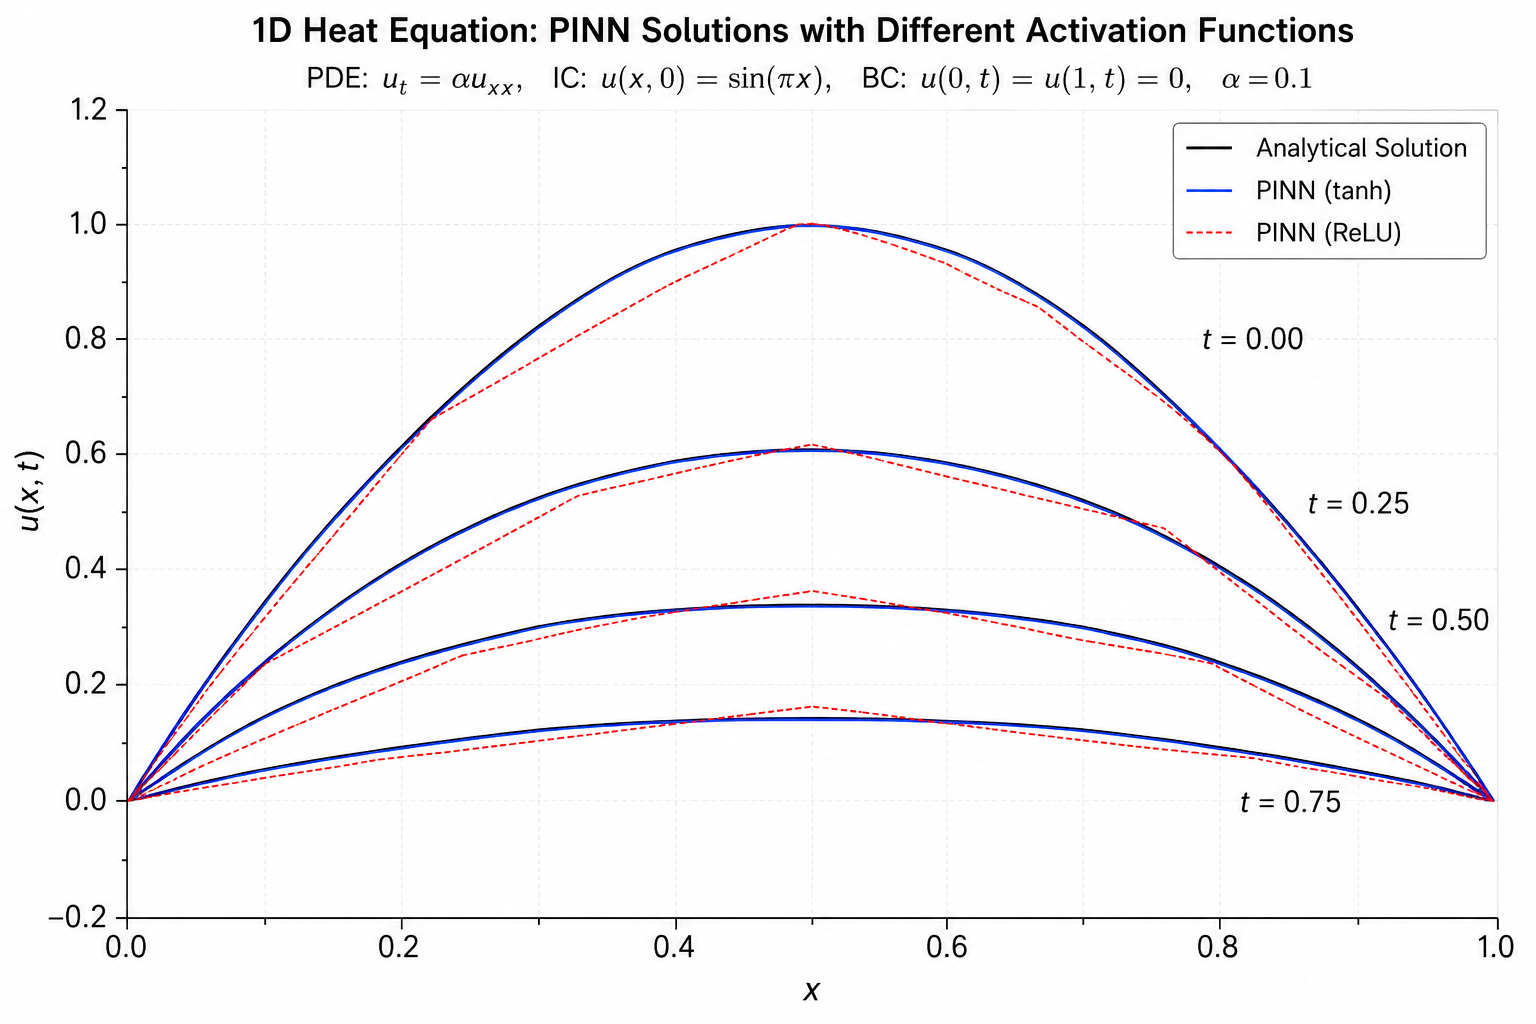
\includegraphics[width=0.75\linewidth]{figures/sol_tanh_vs_relu.png}
    \caption{Comparison of the derivatives of the \texttt{tanh} and \texttt{swish} activation functions.}
    \label{fig:sol_activation}
\end{figure}

Since PINNs require repeated computation of spatial and temporal derivatives through automatic differentiation, smooth activation functions are particularly important.

% =========================================================
\subsection{Automatic Differentiation}
% =========================================================

A central component of the PINN framework is automatic differentiation. Rather than approximating derivatives numerically using finite differences, derivatives are computed analytically through the computational graph of the neural network.

This allows direct evaluation of PDE residuals such as:

\begin{equation}
R(x,t)
=
\frac{\partial T_{\theta}}{\partial t}
-
\alpha
\frac{\partial^2 T_{\theta}}{\partial x^2}
\end{equation}

Automatic differentiation provides highly accurate derivative evaluations and enables efficient optimization of physics-based constraints.

In this work, automatic differentiation is performed using the JAX framework.

% =========================================================
\subsection{Weight Initialization Strategy}
% =========================================================

The initialization of neural network parameters plays a crucial role in the training dynamics and convergence behavior of Physics-Informed Neural Networks (PINNs).

Poor initialization may lead to:
\begin{itemize}
    \item vanishing gradients,
    \item exploding gradients,
    \item unstable optimization,
    \item slow convergence,
    \item or failure to satisfy the PDE constraints.
\end{itemize}

Because PINNs require repeated computation of higher-order derivatives through automatic differentiation, initialization becomes even more important than in standard supervised learning problems.

In this work, the network weights are primarily initialized using the Glorot uniform initialization method, also known as Xavier uniform initialization.

% =========================================================
\subsubsection{Glorot Uniform Initialization}
% =========================================================

The Glorot initialization strategy was introduced to maintain approximately constant variance of activations and gradients throughout the neural network layers during forward and backward propagation.

For a layer containing:
\begin{itemize}
    \item $n_{in}$ input neurons,
    \item and $n_{out}$ output neurons,
\end{itemize}

the weights are initialized from a uniform distribution:

\begin{equation}
W
\sim
\mathcal{U}
\left(
-\sqrt{\frac{6}{n_{in}+n_{out}}},
\sqrt{\frac{6}{n_{in}+n_{out}}}
\right)
\end{equation}

where:
\begin{itemize}
    \item $\mathcal{U}$ denotes the uniform distribution,
    \item and the bounds are chosen to preserve variance stability across layers.
\end{itemize}

This initialization helps prevent:
\begin{itemize}
    \item signal amplification,
    \item signal attenuation,
    \item and unstable gradient propagation.
\end{itemize}

% =========================================================
\subsubsection{Importance for PINNs}
% =========================================================

The Glorot initialization is particularly well suited for PINNs using smooth activation functions such as \texttt{tanh}.

Since PINNs rely heavily on:
\begin{itemize}
    \item automatic differentiation,
    \item PDE residual computation,
    \item and higher-order derivatives,
\end{itemize}

poor initialization may rapidly produce:
\begin{itemize}
    \item nearly constant outputs,
    \item saturated activations,
    \item or unstable PDE residuals.
\end{itemize}

For example, if the weights are initialized with excessively large values, the \texttt{tanh} activation function may rapidly saturate:

\begin{equation}
\tanh(z)
\rightarrow
\pm 1
\end{equation}

leading to near-zero gradients and difficult optimization.

Conversely, excessively small initial weights may produce weak gradients and very slow learning.

The Glorot initialization provides a good compromise by maintaining stable activation amplitudes throughout the network during the early stages of training.

This is especially important for PINNs because:
\begin{itemize}
    \item PDE residual optimization is already highly stiff,
    \item multiple loss terms must be balanced simultaneously,
    \item and inverse parameter estimation problems are particularly sensitive to optimization stability.
\end{itemize}

% =========================================================
\subsubsection{Alternative Initialization Methods}
% =========================================================

Several alternative initialization strategies exist and may also be used depending on the activation functions and problem characteristics.

\paragraph{He Initialization}

He initialization is commonly used for ReLU-based neural networks.

The weights are initialized according to:

\begin{equation}
W
\sim
\mathcal{N}
\left(
0,
\frac{2}{n_{in}}
\right)
\end{equation}

or its uniform equivalent.

This initialization is designed to compensate for the asymmetric behavior of ReLU activations.

However, ReLU activations are generally less suitable for PINNs because:
\begin{itemize}
    \item they are not smooth,
    \item their second derivatives vanish almost everywhere,
    \item and PDE residual computation becomes less accurate.
\end{itemize}

% =========================================================
\paragraph{LeCun Initialization}
% =========================================================

LeCun initialization is often associated with activation functions such as SELU.

It uses:

\begin{equation}
W
\sim
\mathcal{N}
\left(
0,
\frac{1}{n_{in}}
\right)
\end{equation}

This initialization can improve stability for certain self-normalizing architectures.

% =========================================================
\paragraph{Random Small Initialization}
% =========================================================

A simpler strategy consists of initializing all weights with small random values.

Although easy to implement, this approach often leads to:
\begin{itemize}
    \item unstable convergence,
    \item poor gradient propagation,
    \item and inconsistent optimization behavior.
\end{itemize}

Such naive initialization methods are generally not robust enough for PINN applications.

% =========================================================
\subsubsection{Initialization and Optimization Dynamics}
% =========================================================

The experiments performed in this work suggest that initialization strongly influences:
\begin{itemize}
    \item convergence speed,
    \item optimization stability,
    \item PDE residual minimization,
    \item and inverse parameter identifiability.
\end{itemize}

In some cases, different random initializations may lead the optimization process toward:
\begin{itemize}
    \item different local minima,
    \item different reconstructed parameters,
    \item or different balances between physics and data losses.
\end{itemize}

This highlights the highly non-convex nature of PINN optimization landscapes.

Careful initialization therefore constitutes an important component of stable and reproducible PINN training strategies.

% =========================================================
\subsection{Collocation Points}
% =========================================================

\subsection{Collocation Points and Sampling Strategies}

One of the major advantages of Physics-Informed Neural Networks is their ability to enforce physical laws throughout the entire spatio-temporal domain, including regions where no experimental measurements are available. While observational data are generally limited to a finite number of measurement locations, the governing partial differential equation can be evaluated at any point of the domain through automatic differentiation.

To achieve this objective, PINNs introduce a set of collocation points distributed throughout the computational domain. These points are not associated with experimental observations. Instead, they are used to evaluate the residual of the governing equation and enforce physical consistency everywhere in the domain.

The residual loss is computed at each collocation point and penalizes violations of the governing equation. For a set of $(N_{col})$ collocation points $((x_i,t_i))$, the physics loss is defined as

\begin{equation}
\mathcal{L}_{phys} = \frac{1}{N_{col}} \sum_{i=1}^{N_{col}} R(x_i,t_i)^2,
\end{equation}

where $(R(x_i,t_i))$ denotes the PDE residual evaluated at the collocation point $((x_i,t_i))$

The number and distribution of collocation points play a critical role in the performance of a PINN. In general, a sufficient number of points is required to ensure that the physical constraints are enforced throughout the domain. However, increasing the number of collocation points also increases the computational cost of training, since the residual and its derivatives must be evaluated at every collocation point during each optimization step.

Several strategies can be used to generate collocation points.

A first possibility consists of using a fixed structured grid. While simple to implement, this approach may lead to an excessive concentration of points along predefined locations. In some situations, the network may learn to satisfy the governing equation primarily at the grid locations while exhibiting poorer accuracy between them.

Purely random sampling generally improves the coverage of the domain and reduces this risk. However, random sampling can occasionally generate clusters of points in certain regions while leaving other regions sparsely sampled, especially when the number of collocation points is limited.

To overcome this limitation, Latin Hypercube Sampling (LHS) is frequently employed in PINN applications. The method divides the domain into multiple subregions and ensures that samples are distributed more uniformly throughout the domain while preserving a degree of randomness. This typically leads to better coverage of the spatio-temporal domain and improved training stability.

In more challenging problems involving boundary layers, sharp gradients, interfaces, or complex geometries, adaptive sampling strategies may also be employed. In these approaches, additional collocation points are progressively introduced in regions where the PDE residual remains large, allowing the network to focus computational effort where it is most needed.

The choice of sampling strategy is also closely related to the optimization algorithm used during training. When using first-order optimizers such as Adam, collocation points can be regenerated periodically or even at every training epoch. Since Adam relies on stochastic gradient updates, it is relatively robust to changes in the sampled points and can benefit from exploring different regions of the domain throughout training.

In contrast, quasi-Newton optimizers such as L-BFGS assume a fixed optimization landscape during the line-search and Hessian approximation procedures. For this reason, the collocation points are typically kept fixed during the entire L-BFGS optimization phase. In this context, Latin Hypercube Sampling often provides an effective compromise between domain coverage and training stability.

The distribution of collocation points ultimately has a significant impact on the convergence behavior, physical consistency, and predictive accuracy of the resulting PINN solution.

\begin{figure}[ht]
\centering
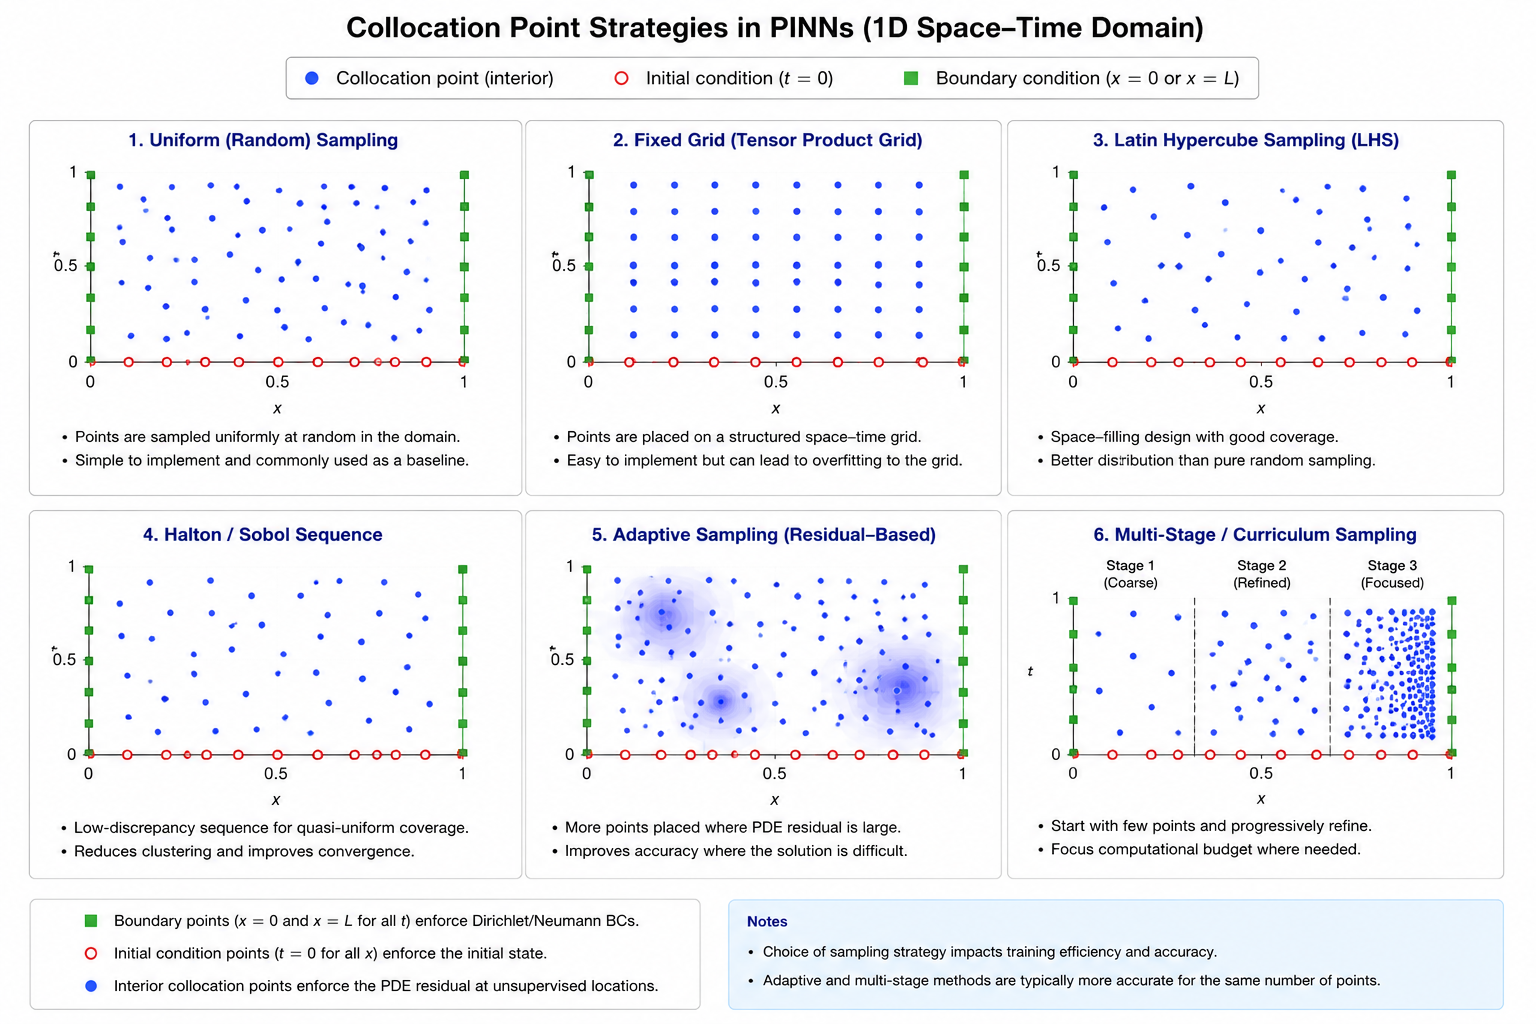
\includegraphics[width=0.75\linewidth]{figures/collocations_pts.png}
\caption{Comparison of common collocation point generation strategies. Uniform grids may lead to poor generalization between sampling locations, purely random sampling may produce clusters and empty regions, whereas Latin Hypercube Sampling provides a more uniform coverage of the spatio-temporal domain.}
\label{fig:collocations_pts}
\end{figure}

\subsection{Boundary and Initial Condition Enforcement}

A Physics-Informed Neural Network must not only satisfy the governing partial differential equation inside the domain, but also the initial and boundary conditions of the physical problem. For the one-dimensional heat diffusion problem considered in this work, the temperature field is defined on the spatial domain $x \in [0,L]$ and the temporal domain $t \in [0,t_{\max}]$. The governing equation is

\begin{equation}
\frac{\partial T}{\partial t} = \alpha \frac{\partial^2 T}{\partial x^2}
\end{equation}

The associated initial and boundary conditions are

\begin{equation}
T(x,0) = T_0(x),
\end{equation}

and

\begin{equation}
T(0,t)=0,
\qquad
T(L,t)=0.
\end{equation}

In this work, the initial condition is chosen as

\begin{equation}
T_0(x) = \sin\left(\frac{\pi x}{L}\right).
\end{equation}

The PINN must therefore produce a temperature field that is consistent with the data, satisfies the heat equation inside the domain, and respects the prescribed initial and boundary conditions.

Two main approaches can be used to impose initial and boundary conditions in PINNs:

\begin{itemize}
\item soft constraints,
\item hard constraints.
\end{itemize}

\subsubsection{Soft Constraint Formulation}

In the soft constraint approach, the initial and boundary conditions are not imposed directly in the structure of the neural network. Instead, they are added as penalty terms in the loss function.

The neural network directly predicts the temperature field as

\begin{equation}
T_{\theta}(x,t) = \mathcal{N}_{\theta}(x,t).
\end{equation}

The physics loss is computed from the PDE residual,

\begin{equation}
R(x,t) =  \frac{\partial T_{\theta}}{\partial t} - \alpha
\frac{\partial^2 T_{\theta}}{\partial x^2}
\end{equation}

For a set of $N_f$ collocation points $(x_i,t_i)$, the physics loss is written as

\begin{equation}
\mathcal{L}_{phys} = \frac{1}{N_f} \sum_{i=1}^{N_f} R(x_i,t_i)^2.
\end{equation}

The initial condition loss is defined by comparing the network prediction at $t=0$ with the prescribed initial profile:

\begin{equation}
\mathcal{L}_{IC} = \frac{1}{N_{IC}} \sum_{i=1}^{N_{IC}} \left[ T_{\theta}(x_i,0) -  T_0(x_i) \right]^2.
\end{equation}

Similarly, the boundary condition loss enforces the temperature at both ends of the domain:

\begin{equation}
\mathcal{L}_{BC} =  \frac{1}{N_{BC}}
\sum_{i=1}^{N_{BC}}
\left[
T_{\theta}(0,t_i)^2 - 0^2
+
T_{\theta}(L,t_i)^2 - 0^2
\right].
\end{equation}

If observational data are available, a data loss can also be added:

\begin{equation}
\mathcal{L}_{data} = 
\frac{1}{N_d}
\sum_{i=1}^{N_d}
\left[
T_{\theta}(x_i,t_i) - T_i^{obs}
\right]^2
\end{equation}

The total loss function is then written as

\begin{equation}
\mathcal{L}_{total} = \lambda_{data}\mathcal{L}_{data}
+
\lambda_{phys}\mathcal{L}_{phys}
+
\lambda_{IC}\mathcal{L}_{IC}
+
\lambda_{BC}\mathcal{L}_{BC}.
\end{equation}

The coefficients $\lambda_{data}$, $\lambda_{phys}$, $\lambda_{IC}$, and $\lambda_{BC}$ control the relative importance of each constraint during training.

This formulation is flexible and useful when the initial or boundary conditions are uncertain, noisy, or only partially known. However, it introduces a trade-off between the different loss terms. If the weighting coefficients are not properly chosen, the network may satisfy the PDE while poorly satisfying the boundary conditions, or conversely fit the initial and boundary conditions while producing a physically inconsistent solution inside the domain.

\subsubsection{Hard Constraint Formulation}

In the hard constraint approach, the initial and boundary conditions are embedded directly into the analytical form of the neural network output. Instead of letting the network freely predict $T_{\theta}(x,t)$, the prediction is constructed using an ansatz that automatically satisfies the prescribed conditions.

For the one-dimensional heat equation with

\begin{equation}
T(x,0) = \sin\left(\frac{\pi x}{L}\right),
\qquad
T(0,t)=0,
\qquad
T(L,t)=0,
\end{equation}

a suitable hard-constrained formulation is

\begin{equation}
T_{\theta}(x,t) =\sin\left(\frac{\pi x}{L}\right)
+
tx(L-x),\mathcal{N}_{\theta}(x,t).
\end{equation}

This expression is commonly referred to as an ansatz. The ansatz is constructed so that the known constraints are automatically satisfied regardless of the values predicted by the neural network.

Indeed, at $t=0$,

\begin{equation}
T_{\theta}(x,0) = \sin\left(\frac{\pi x}{L}\right)
+
0 \cdot x(L-x)\mathcal{N}_{\theta}(x,0),
\end{equation}

which gives

\begin{equation}
T_{\theta}(x,0) = 
\sin\left(\frac{\pi x}{L}\right).
\end{equation}

The initial condition is therefore satisfied exactly.

Similarly, at $x=0$,

\begin{equation}
T_{\theta}(0,t) = \sin(0)
+
t \cdot 0 \cdot L \cdot \mathcal{N}_{\theta}(0,t) = 0,
\end{equation}

and at $x=L$,

\begin{equation}
T_{\theta}(L,t) = \sin(\pi) + t \cdot L \cdot (L-L) \cdot \mathcal{N}_{\theta}(L,t) = 0
\end{equation}

The boundary conditions are therefore also satisfied exactly for every value of $t$.

Because the initial and boundary conditions are already enforced by construction, the corresponding loss terms are no longer required. The total loss function becomes

\begin{equation}
\mathcal{L}_{total} = \lambda_{data}\mathcal{L}_{data} + \lambda_{phys}\mathcal{L}_{phys}.
\end{equation}

The optimization process can therefore focus entirely on minimizing the data loss and the physics residual.

\subsubsection{Comparison Between Soft and Hard Constraints}

Soft constraints are simple to implement and provide flexibility when the prescribed conditions are uncertain or noisy. However, they require careful tuning of multiple weighting coefficients and may not enforce the conditions with high accuracy.

Hard constraints require the construction of an appropriate ansatz adapted to the problem under consideration. Although this introduces additional analytical work, the initial and boundary conditions are satisfied exactly throughout training.

For benchmark problems where the conditions are known precisely, hard constraints generally improve numerical accuracy, reduce the number of competing loss terms, and simplify the optimization problem. For this reason, the hard-constrained formulation is adopted throughout most of the present study.


% =========================================================
\subsection{Optimization Strategy}
% =========================================================

Training a PINN corresponds to solving a high-dimensional nonlinear optimization problem.

In this work, optimization is primarily performed using the Limited-memory Broyden–Fletcher–Goldfarb–Shanno (L-BFGS) algorithm implemented through the \texttt{jaxopt} library.

L-BFGS is particularly attractive for PINN applications because:
\begin{itemize}
    \item it provides fast convergence on smooth optimization problems,
    \item it efficiently exploits second-order curvature information,
    \item and it often converges more reliably than stochastic gradient-based optimizers for PDE-constrained learning.
\end{itemize}

The optimization process iteratively updates the network parameters in order to minimize the global loss function.

\begin{figure}
    \centering
    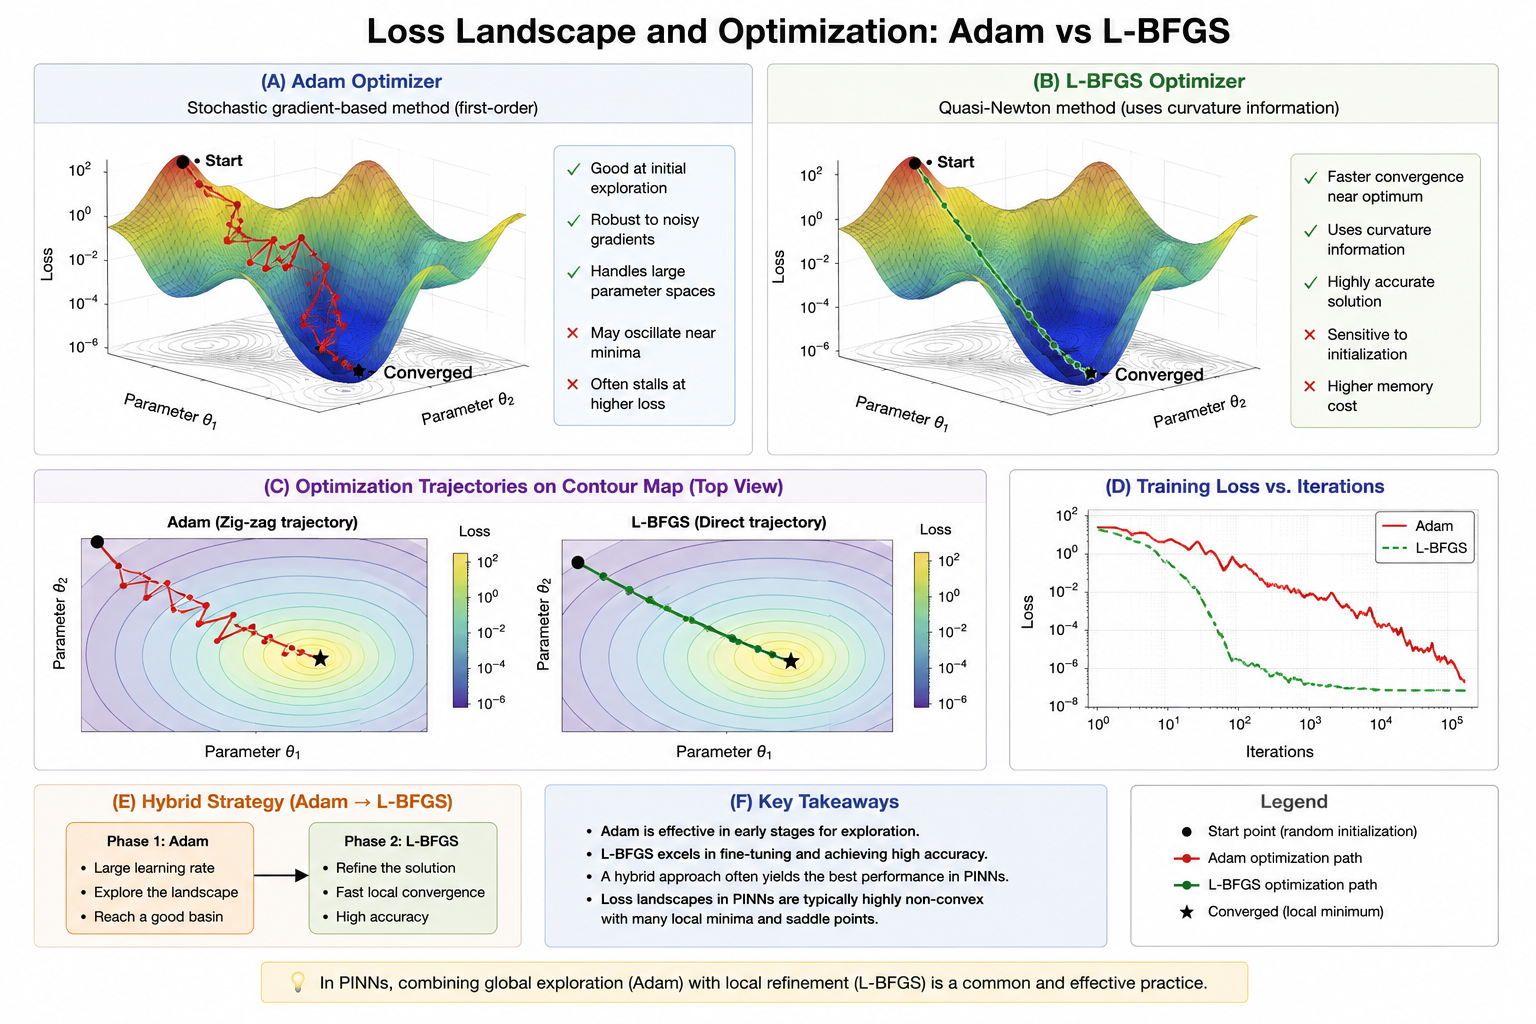
\includegraphics[width=0.75\linewidth]{figures/adam_vs_LBFGS.png}
    \caption{Comparison between \texttt{adam} and \texttt{LBFGS} optimizers}
    \label{fig:adam vs LBFGS}
\end{figure}

% =========================================================
\subsection{Floating Point Precision}
% =========================================================

PINNs can be sensitive to numerical precision, especially when computing higher-order derivatives or balancing multiple loss terms with different magnitudes.

For this reason, computations in this work are performed using double precision (\texttt{float64}) rather than single precision (\texttt{float32}).

This improves:
\begin{itemize}
    \item numerical stability,
    \item derivative accuracy,
    \item and optimization robustness.
\end{itemize}

% =========================================================
\subsection{Random Seeds and Reproducibility}
% =========================================================

Reproducibility is an important aspect of Physics-Informed Neural Network (PINN) research. Unlike deterministic numerical solvers, PINN training involves several stochastic components that may significantly influence:
\begin{itemize}
    \item convergence behavior,
    \item optimization stability,
    \item final solution accuracy,
    \item and inverse parameter reconstruction.
\end{itemize}

For this reason, careful management of random seeds is essential in order to obtain reproducible and interpretable results.

In this work, several independent sources of randomness were identified and controlled separately.

% =========================================================
\subsubsection{Weight Initialization Seed}
% =========================================================

The first important source of randomness concerns neural network weight initialization.

Since the network parameters are initialized randomly using methods such as Glorot uniform initialization, different seeds produce different initial optimization trajectories.

This may strongly affect:
\begin{itemize}
    \item convergence speed,
    \item local minima selection,
    \item PDE residual minimization,
    \item and inverse parameter estimation.
\end{itemize}

Even when all hyperparameters remain identical, two different initialization seeds may lead to significantly different final solutions due to the highly non-convex nature of the PINN optimization landscape.

For this reason, the initialization seed must always be controlled and reported.

% =========================================================
\subsubsection{Collocation Point Seed}
% =========================================================

A second important source of randomness concerns the generation of collocation points used to evaluate the PDE residual.

In this work, collocation points are typically generated using Latin Hypercube Sampling (LHS).

Different seeds therefore produce different spatial and temporal point distributions inside the domain.

This directly influences:
\begin{itemize}
    \item PDE residual evaluation,
    \item domain coverage,
    \item optimization stability,
    \item and parameter identifiability.
\end{itemize}

For inverse problems, collocation point placement can become particularly important because:
\begin{itemize}
    \item some regions contain significantly more information regarding the unknown parameter $\alpha$,
    \item while other regions may contribute little useful information.
\end{itemize}

Consequently, collocation seeds may substantially affect inverse reconstruction quality.

% =========================================================
\subsubsection{Dataset Generation Seed}
% =========================================================

Another critical source of randomness concerns synthetic dataset generation.

Noisy observations are generated by adding random perturbations to the analytical solution:

\begin{equation}
T_{obs}
=
T_{exact}
+
\varepsilon
\end{equation}

where $\varepsilon$ represents random noise.

Different dataset seeds therefore generate different noisy realizations of the same physical problem.

This may influence:
\begin{itemize}
    \item the signal-to-noise ratio,
    \item the effective information content,
    \item and the difficulty of the inverse problem.
\end{itemize}

In some configurations, specific noise realizations may strongly degrade parameter identifiability.

For this reason, robustness studies should not rely on a single dataset realization.

% =========================================================
\subsubsection{Training and Optimization Randomness}
% =========================================================

Additional stochasticity may also appear during optimization depending on:
\begin{itemize}
    \item minibatch selection,
    \item hardware execution order,
    \item floating point precision,
    \item parallel execution,
    \item and framework-specific nondeterministic operations.
\end{itemize}

Although deterministic optimizers such as L-BFGS reduce part of this variability, numerical differences may still emerge depending on:
\begin{itemize}
    \item compilation,
    \item execution backend,
    \item and machine architecture.
\end{itemize}

This is particularly relevant when using:
\begin{itemize}
    \item GPU acceleration,
    \item JIT compilation,
    \item or highly optimized automatic differentiation libraries.
\end{itemize}

% =========================================================
\subsubsection{Importance of Multi-Seed Robustness Studies}
% =========================================================

The experiments performed in this work showed that PINN performance may vary significantly depending on the selected seeds.

A single successful run is therefore insufficient to evaluate the robustness of a PINN methodology.

For this reason, robustness studies were systematically conducted using multiple:
\begin{itemize}
    \item initialization seeds,
    \item dataset seeds,
    \item and collocation point seeds.
\end{itemize}

This allows:
\begin{itemize}
    \item estimation of variability across runs,
    \item identification of unstable training configurations,
    \item and more reliable evaluation of inverse reconstruction performance.
\end{itemize}

Such analyses are particularly important for inverse problems where optimization landscapes are highly non-convex and sensitive to small perturbations.

% =========================================================
\subsubsection{Seed Management in Practice}
% =========================================================

In practice, careful seed management requires:
\begin{itemize}
    \item explicit initialization of random number generators,
    \item independent control of different randomness sources,
    \item and systematic recording of seed values for reproducibility.
\end{itemize}

Typical controlled seeds in this work include:
\begin{itemize}
    \item neural network initialization seeds,
    \item collocation sampling seeds,
    \item noisy dataset generation seeds,
    \item and experiment-level global seeds.
\end{itemize}

This reproducibility strategy is essential for:
\begin{itemize}
    \item fair comparison between experiments,
    \item reliable hyperparameter studies,
    \item and rigorous evaluation of PINN robustness.
\end{itemize}

% =========================================================
\subsection{Role of the Forward PINN Benchmark}
% =========================================================

Although the forward heat diffusion problem is relatively simple and classical numerical solvers remain significantly more efficient for this type of simulation, studying the forward PINN problem remains highly valuable.

The forward benchmark provides a controlled environment for understanding:
\begin{itemize}
    \item how PINNs learn physical constraints,
    \item how optimization behaves under different hyperparameter choices,
    \item how data and physics losses interact,
    \item and how numerical pathologies may emerge during training.
\end{itemize}

This understanding is essential before addressing more challenging inverse problems or extending the methodology toward nonlinear PDEs, complex geometries, multiphysics systems, or real experimental datasets.